\documentclass[11pt,a4paper]{article}

% ---------- Packages ----------
\usepackage[utf8]{inputenc}
\usepackage[T1]{fontenc}
\usepackage{lmodern}
\usepackage[margin=1in]{geometry}
\usepackage{amsmath,amssymb,amsfonts}
\usepackage{graphicx}
\usepackage{booktabs}
\usepackage{multirow}
\usepackage{array}
\usepackage{float}
\usepackage{caption}
\usepackage{subcaption}
\usepackage{siunitx}
\usepackage{hyperref}
\usepackage[numbers,sort&compress]{natbib}
\usepackage{xcolor}
\usepackage{authblk}
\usepackage{microtype}
\usepackage{enumitem}
\usepackage{tabularx}

\hypersetup{
  colorlinks=true,
  linkcolor=black,
  citecolor=blue,
  urlcolor=blue
}

% ---------- Custom macros ----------
\newcommand{\nppad}{NPPAD\xspace}
\newcommand{\todo}[1]{\textcolor{red}{[TODO: #1]}}
\newcommand{\placeholder}[1]{\textcolor{orange}{[#1]}}
\usepackage{xspace}

% ---------- Title ----------
\title{\textbf{An Integrated Deep Learning Framework for Nuclear Reactor Fault Diagnosis: From Semi-Supervised Anomaly Detection to Physics-Informed Accident Prognosis}}

\author[1]{Romeo Nickel}
\affil[1]{\textit{Affiliation TBD}}

\date{\today}

\begin{document}
\maketitle

\begin{abstract}
Reliable fault diagnosis in nuclear power plants requires a cascading chain of decisions: detecting that an anomaly has occurred, identifying what type of accident is underway, and predicting how the reactor state will evolve. Existing machine learning approaches for nuclear fault diagnosis typically address these tasks independently, limiting their utility for integrated digital-twin deployments where diagnostic outputs must be physically consistent across stages. This paper presents a unified three-stage deep learning framework for pressurized water reactor (PWR) fault diagnosis, evaluated on the Nuclear Power Plant Accident Dataset (\nppad) comprising 96 sensor parameters across 18 operating conditions. In the first stage, semi-supervised anomaly detectors (autoencoder, LSTM, and Transformer) trained exclusively on normal operating data achieve near-perfect detection performance ($\mathrm{F1} \approx 0.9995$, $\mathrm{AUROC} \geq 0.985$) on 7{,}316 test windows. In the second stage, a bidirectional LSTM classifier identifies the specific accident type with $71.2\%$ accuracy across 18 classes, with SHAP-based attribution analysis providing per-sensor and per-timestep root-cause information. In the third stage, a physics-informed GRU encoder--decoder surrogate ($384$K parameters), constrained by point kinetics equations and energy conservation laws, predicts 10-step reactor trajectories with $68.6\%$ lower point-kinetics residuals and $39.6\%$ fewer energy-conservation violations than an otherwise-identical data-only baseline. The integration of these stages enables a complete diagnostic pipeline in which physics-informed predictions cross-validate data-driven classifications, demonstrating a viable architecture for nuclear digital-twin monitoring systems.
\end{abstract}

\noindent\textbf{Keywords:} nuclear power plant, fault diagnosis, anomaly detection, physics-informed neural network, digital twin, SHAP, deep learning, pressurized water reactor

\section{Introduction}
\label{sec:introduction}

The safe operation of a nuclear power plant depends on a control-room decision process that cascades across three questions in rapid succession. First, the operator must decide whether plant behaviour has departed from normal operating conditions at all. Second, if a departure has occurred, its type must be identified: a loss-of-coolant accident (LOCA), a steam-generator tube rupture (SGTR), a main steam line break (MSLB), and many other failure modes evolve with distinct physical signatures and demand different emergency operating procedures. Third, the operator must anticipate how the plant will evolve over the next several minutes so that mitigating actions can be selected before safety limits are challenged. Each of these questions maps onto an established class of data-driven problems---anomaly detection, multi-class classification, and time-series forecasting---but in practice they are rarely addressed as a coordinated system.

Most machine-learning studies on nuclear fault diagnosis focus on a single stage of this chain. Purely data-driven classifiers achieve strong in-distribution accuracy on simulator data but can produce predictions that are inconsistent with reactor physics when deployed on out-of-distribution transients~\citep{qi2022nppad,zhang2023pinn,santhosh2019survey}. Surrogate reactor models trained with physics-informed losses can preserve conservation laws but are typically evaluated as stand-alone models rather than as components of a broader diagnostic system~\citep{raissi2019pinn,zhang2023pinn,gong2022rom}. Recent digital-twin review articles explicitly call for integrated monitoring--diagnosis--prognosis architectures~\citep{ayodeji2022dtwin,digitaltwin2025review}, yet few published works deliver concrete implementations that span the full chain.

This paper contributes such an implementation. We build a three-stage deep-learning framework for PWR fault diagnosis on the open-source Nuclear Power Plant Accident Dataset (\nppad)~\citep{qi2022nppad}, which provides 96 sensor channels across 18 operating conditions generated by the PCTRAN PWR simulator. The three stages and their design rationale are summarized as follows:

\begin{enumerate}[leftmargin=*]
    \item \textbf{Semi-supervised anomaly detection.} We train three architectures (autoencoder, LSTM next-step predictor, masked Transformer reconstructor) on normal operating data only, reflecting the practical reality that accident data at a real plant is scarce, simulated, or both. Anomaly scores are thresholded on validation data. This stage acts as a broad screening gate.
    \item \textbf{Multi-class accident classification with root-cause attribution.} We compare a 1D-CNN, a bidirectional LSTM, and a Transformer with a learnable classification token on the 18-class problem, and we apply SHAP and input $\times$ gradient attribution to the best-performing model to recover per-sensor and per-timestep importance scores. Crucially, we interpret these scores against the known physics of each accident type: for well-understood classes such as LOCA, SLB, and SGTR, we check whether the attributions highlight the sensors predicted by the underlying physical mechanism.
    \item \textbf{Physics-informed trajectory prediction.} We train a GRU encoder--decoder surrogate with a composite loss that combines mean-squared trajectory error, a point-kinetics residual, an energy-conservation residual, and physical-bounds penalties. The surrogate predicts ten time steps ahead from a twenty-step context window, allowing us to generate a short-horizon forecast that can be compared against the observed trajectory as a physics-grounded consistency check.
\end{enumerate}

The central novelty of the paper is not any single stage but the way they are composed. Each stage addresses a distinct question, and the output of one stage conditions the input to the next. More importantly, the physics-informed surrogate of stage three provides a mechanism by which the diagnostic outputs of stages one and two can be cross-validated against reactor physics: if the predicted trajectory conditioned on a classifier's decision is physically inconsistent with what actually unfolds, the classification can be flagged as low-confidence. This cross-validation loop is, to our knowledge, absent from prior published work on \nppad{}.

Our contributions are:

\begin{itemize}[leftmargin=*]
    \item A reproducible three-stage fault diagnosis pipeline on \nppad{} covering anomaly detection, 18-class accident classification, and physics-constrained trajectory prediction, with open configurations and training scripts.
    \item A quantitative evaluation showing that three independent anomaly-detection architectures achieve near-perfect screening ($\mathrm{F1} \approx 0.9995$), that a bidirectional LSTM is the strongest classifier with $71.2\%$ accuracy and $0.572$ macro-F1 on the imbalanced 18-class problem, and that embedding point kinetics and energy conservation into the surrogate's loss reduces physics residuals by $68.6\%$ and energy-conservation violations by $39.6\%$ relative to an unconstrained baseline.
    \item A physics-grounded interpretation of SHAP attributions for representative accident classes, establishing that the classifier's decision process is aligned with mechanistic knowledge of the underlying transients.
    \item A pipeline-integration analysis showing how physics-informed predictions can serve as a consistency check on data-driven classifications, together with a discussion of the conditions under which such cross-validation is most informative.
\end{itemize}

The remainder of the paper is organized as follows. Section~\ref{sec:related} reviews related work. Section~\ref{sec:method} describes each of the three stages and their integration. Section~\ref{sec:setup} details the experimental protocol. Section~\ref{sec:results} presents quantitative and qualitative results. Section~\ref{sec:discussion} discusses limitations and generalization to real plants and advanced reactor designs. Section~\ref{sec:conclusion} concludes.

\section{Related Work}
\label{sec:related}

\subsection{Data-Driven Fault Diagnosis in Nuclear Plants}

Machine-learning approaches to nuclear fault diagnosis have evolved from classical pattern-recognition methods to deep sequence models. Early work used feed-forward networks and support vector machines on static snapshots of sensor data, and was reviewed comprehensively by Santhosh~et~al.~\citep{santhosh2019survey}. The release of the open-source Nuclear Power Plant Accident Dataset~\citep{qi2022nppad} enabled the systematic benchmarking of modern sequence architectures. Subsequent studies applied convolutional and recurrent networks to the 18-class accident identification problem, reporting high in-distribution accuracy for common transients but persistent difficulties with rare or physically similar accident types~\citep{wang2023deep,lee2023lstm}.

More recent work has turned to explainability. A January 2026 study by \placeholder{Author et al.}~\citep{xgboost2026shap} combined SHAP-based feature attribution with an incremental XGBoost classifier on a \nppad-derived feature set, using SHAP primarily for feature selection and incremental model updating. Our work differs in two ways. First, we operate on raw multivariate windows rather than hand-engineered feature summaries, retaining the temporal structure that downstream prognosis requires. Second, we use SHAP not as a feature-selection heuristic but as a physics-grounded root-cause-attribution tool---validating that the classifier's attributions align with the known mechanistic signatures of each accident type---and we fold the attribution analysis into a broader pipeline rather than treating it as a standalone result.

\subsection{Physics-Informed Machine Learning for Nuclear Systems}

Physics-informed neural networks (PINNs) augment data-driven objectives with residuals from governing partial or ordinary differential equations~\citep{raissi2019pinn,karniadakis2021pinn}. In the nuclear domain, PINNs have been applied to reactor transient prediction~\citep{zhang2023pinn}, autonomous core calibration~\citep{song2023calibration}, and reduced-order modeling within digital-twin workflows~\citep{gong2022rom}. These studies demonstrate that embedding reactor physics (point kinetics, two-phase flow closures, or full neutron transport) improves generalization to regimes with limited training data.

Our physics-informed surrogate follows this tradition but differs in its embedding scope and pipeline role. We embed point kinetics and steady-state energy conservation constraints---rather than a full neutron-transport operator---because our target is a \emph{plant-level} surrogate covering 96 coupled sensor channels rather than a detailed core model. More importantly, our surrogate is designed from the outset as the third stage of a diagnostic pipeline; its outputs are used as consistency checks on the classifier, not only as physically plausible forecasts in their own right.

\subsection{Digital Twins and Integrated Pipelines for NPPs}

The digital-twin paradigm for nuclear plants has been the subject of several recent review articles~\citep{ayodeji2022dtwin,digitaltwin2025review}, which converge on a monitoring--diagnosis--prognosis architecture as the natural software organization for safety-relevant decision support. These reviews emphasize, however, that few published works actually implement the full chain: most demonstrations terminate at classification, and the prognosis stage is often treated as future work. Where prognosis is addressed, it is typically a purely data-driven forecaster without explicit physics constraints, which makes its predictions difficult to trust for out-of-distribution transients or unseen accident severities.

Our contribution is a concrete implementation of the monitoring--diagnosis--prognosis chain on a public dataset, with explicit physics constraints in the prognosis stage and an attribution layer in the diagnosis stage that ties model decisions back to mechanistic knowledge. This makes the system interpretable at the level of individual predictions and auditable at the level of physical consistency, both of which are prerequisites for regulated deployment.

\section{Methodology}
\label{sec:method}

Figure~\ref{fig:pipeline} gives a schematic overview of the integrated framework. A sliding window of 30 time steps over the 96 sensor channels is the common input representation. Stage 1 produces a binary anomaly flag, stage 2 produces an 18-class accident label plus per-sensor and per-timestep attributions, and stage 3 produces a ten-step forward trajectory prediction along with the scalar physics residuals attached to that prediction. The downstream consistency check combines the stage-2 label with the stage-3 trajectory, as detailed in Section~\ref{sec:integration}.

\begin{figure}[H]
    \centering
    \placeholder{Figure 1: pipeline schematic. Boxes for modules 1--3 with arrows showing data flow; inset showing the cross-validation check between module 2 and module 3.}
    \caption{Overview of the three-stage integrated framework. Stage 1 performs semi-supervised screening on normal-data-trained models. Stage 2 performs supervised 18-class classification with SHAP attribution. Stage 3 produces physics-informed short-horizon trajectory predictions that can be cross-checked against the stage-2 classification.}
    \label{fig:pipeline}
\end{figure}

\subsection{Data Representation}
\label{sec:data-rep}

Raw \nppad{} recordings are resampled onto a uniform time grid and concatenated into per-scenario sequences of $96$ sensor channels covering primary-loop pressures, hot/cold-leg temperatures, coolant flow rates, reactor power, neutron flux, pressurizer level, steam generator levels and pressures, and boron concentration. Sequences are split by scenario into $70/15/15$ train/validation/test partitions to avoid leakage within a single transient. A standard scaler is fit on the normal-operation training subset only, and applied to all partitions.

Sliding windows of length $T = 30$ time steps are drawn with stride $s_{\text{train}} = 10$ during training and $s_{\text{eval}} = 1$ during evaluation, yielding $32{,}284$ training windows and $7{,}316$ test windows. Each window is labelled with both a binary anomaly flag and the 18-way accident-type label of its parent scenario.

\subsection{Stage 1: Semi-Supervised Anomaly Detection}
\label{sec:anomaly}

Stage 1 comprises three architectures trained only on the 28 normal-operation windows in the training set. Anomaly scores are derived from reconstruction or prediction error, and a decision threshold is tuned on validation data to maximize F1.

\paragraph{Autoencoder.} A fully connected encoder--decoder with layer widths $96 \rightarrow 64 \rightarrow 32 \rightarrow 16 \rightarrow 32 \rightarrow 64 \rightarrow 96$, ReLU activations, and batch normalization reconstructs each timestep independently. The anomaly score for a window is the mean per-timestep mean-squared reconstruction error.

\paragraph{LSTM next-step predictor.} A bidirectional LSTM with hidden size 128 is trained with teacher forcing to predict timestep $t+1$ from timesteps $1{:}t$. The anomaly score is the mean squared prediction error across the window.

\paragraph{Masked Transformer reconstructor.} A Transformer encoder with sinusoidal positional encoding, three layers, and eight attention heads reconstructs a randomly masked $15\%$ of the timesteps in each training window. At inference, the model is asked to reconstruct every timestep, and the mean reconstruction error is used as the anomaly score.

All three models are trained with Adam, a learning rate of $10^{-3}$, early stopping on validation loss with patience 10, and a batch size of 64.

\subsection{Stage 2: Accident Classification with Root-Cause Attribution}
\label{sec:classifier}

Stage 2 is a supervised 18-class classifier operating on the same 30-step window representation. We train three architectures to assess how inductive bias affects performance on this imbalanced problem.

\paragraph{1D-CNN classifier.} Three convolutional blocks ($96\rightarrow 64 \rightarrow 128 \rightarrow 256$ channels, kernel size 3, ReLU, batch normalization) feed into a global average pooling layer, a 128-unit fully connected layer, and an 18-way softmax head. Dropout of $0.3$ is applied before the final layer.

\paragraph{Bidirectional LSTM classifier.} A two-layer bidirectional LSTM with hidden size 128 is unrolled over the 30-step window. The final hidden states from both directions are concatenated ($256$ units), passed through a 128-unit fully connected layer with dropout, and then into the softmax head.

\paragraph{Transformer classifier.} A learnable \texttt{[CLS]} token is prepended to the window, positional encodings are added, and three encoder layers (model dimension 128, eight heads, feed-forward dimension 512) attend over the sequence. The final \texttt{[CLS]} representation is passed through LayerNorm, a 128-unit linear layer with ReLU and dropout, and the softmax head.

All classifiers are trained with cross-entropy loss, Adam, early stopping with patience 15, and learning rates $10^{-3}$ for CNN/LSTM and $5 \times 10^{-4}$ for the Transformer.

\paragraph{Root-cause attribution.} We compute two complementary attribution signals on the best-performing classifier. SHAP values~\citep{lundberg2017shap} are computed with the \texttt{DeepExplainer} backend using a 100-window background sample drawn from the training set. This yields a per-sample tensor of shape $(T \times F)$ assigning an importance score to every (timestep, sensor) pair. We additionally compute input-$\times$-gradient attributions as a faster alternative for large-scale analyses. Per-class feature importance is obtained by averaging absolute SHAP values over all test samples of that class; per-class temporal importance is obtained by averaging over sensors. In Section~\ref{sec:results-shap} we map the top-ranked sensors of representative classes onto physical parameter groups (primary pressure, coolant flow, steam generator secondary side, \textit{etc.}) and compare against the known mechanistic signature of each accident.

\subsection{Stage 3: Physics-Informed Trajectory Prediction}
\label{sec:pinn}

Stage 3 is a GRU encoder--decoder surrogate trained under a composite physics-informed loss. Given a context window of $T_c = 20$ time steps, the model predicts the next $T_p = 10$ time steps of all 96 sensor channels.

\subsubsection{Architecture}

The encoder is a two-layer GRU with hidden size 128 that ingests the context window and produces a final hidden state $\mathbf{h}_{T_c}$. The decoder is an autoregressive GRU initialized from $\mathbf{h}_{T_c}$ that emits, at each decode step $k = 1, \dots, T_p$, a delta vector $\Delta \hat{\mathbf{x}}_k \in \mathbb{R}^{96}$ via a linear projection. The predicted state is obtained by a residual connection
\begin{equation}
    \hat{\mathbf{x}}_{T_c + k} = \mathbf{x}_{T_c} + \sum_{j = 1}^{k} \Delta \hat{\mathbf{x}}_j,
    \label{eq:residual}
\end{equation}
which biases the model towards the local linearization of the dynamics and stabilizes autoregressive roll-outs. The total parameter count is $384$K, small enough for real-time inference on a CPU.

\subsubsection{Physics-Informed Loss}

The training loss combines four terms:
\begin{equation}
    \mathcal{L}(\theta) = \lambda_{\text{data}} \mathcal{L}_{\text{data}} + w(t)\bigl[\lambda_{\text{pk}} \mathcal{L}_{\text{pk}} + \lambda_{\text{cons}} \mathcal{L}_{\text{cons}}\bigr] + \lambda_{\text{bnd}} \mathcal{L}_{\text{bnd}},
    \label{eq:loss}
\end{equation}
where $w(t)$ is a linear warmup schedule ramping from $0$ to $1$ over the first $500$ training steps. We set $\lambda_{\text{data}} = 1.0$, $\lambda_{\text{pk}} = 0.1$, $\lambda_{\text{cons}} = 0.05$, $\lambda_{\text{bnd}} = 0.01$.

\paragraph{Data term.} $\mathcal{L}_{\text{data}}$ is the mean-squared error between predicted and true sensor trajectories in the standard-scaler-normalized space.

\paragraph{Point-kinetics residual.} Let $n(t)$ denote the predicted neutron density channel and let $T_{\text{avg}}(t)$ and $C_{\text{B}}(t)$ denote the predicted coolant average temperature and boron concentration. A simplified point kinetics model assumes
\begin{equation}
    \frac{dn}{dt} = \frac{\rho(t)}{\Lambda} n(t),
    \qquad
    \rho(t) = \alpha_T (T_{\text{avg}}(t) - T_{\text{ref}}) + \alpha_B (C_{\text{B}}(t) - C_{\text{B,ref}}),
    \label{eq:point-kinetics}
\end{equation}
with prompt neutron generation time $\Lambda = 2.0 \times 10^{-5}$~s, temperature coefficient $\alpha_T = -2.0 \times 10^{-4}$~$\Delta k/k$/\textdegree{}C, boron coefficient $\alpha_B = -1.0 \times 10^{-4}$~$\Delta k/k$/ppm, reference temperature $T_{\text{ref}} = 310$~\textdegree{}C, and reference boron concentration $C_{\text{B,ref}} = 200$~ppm, consistent with standard large-PWR parameters~\citep{duderstadt1976nuclear}. The residual is the squared error between the finite-difference time derivative of the predicted $n(t)$ and the right-hand side of Eq.~\eqref{eq:point-kinetics} evaluated on the prediction, averaged over the prediction horizon and normalized by a characteristic neutron density scale.

\paragraph{Energy-conservation residual.} At steady state, core thermal power $Q$ is related to primary loop flow $W$, coolant specific heat $c_p = 5.5$~kJ/kg/\textdegree{}C, and the hot/cold leg temperature difference $\Delta T = T_{\text{hot}} - T_{\text{cold}}$ via
\begin{equation}
    Q \approx W \, c_p \, \Delta T.
    \label{eq:conservation}
\end{equation}
Using the predicted values of $Q$, $W$, $T_{\text{hot}}$, and $T_{\text{cold}}$, $\mathcal{L}_{\text{cons}}$ is the squared residual of Eq.~\eqref{eq:conservation} normalized by a characteristic power scale. During rapid transients Eq.~\eqref{eq:conservation} does not hold exactly, but its inclusion as a soft penalty biases the surrogate towards quasi-steady energy balance, which is physically correct on sufficiently long time scales.

\paragraph{Physical-bounds penalty.} For each channel in a predefined set (pressures, power, temperatures, flow rates, boron concentration), $\mathcal{L}_{\text{bnd}}$ applies a one-sided quadratic penalty whenever the prediction falls below the physically admissible floor.

\subsubsection{Solver}

Where the point-kinetics residual is integrated rather than differentiated during evaluation, we use a fully differentiable fourth-order Runge--Kutta integrator implemented in PyTorch, enabling gradient flow through physical rollouts if desired for future extensions.

\subsection{Pipeline Integration and Cross-Validation}
\label{sec:integration}

At deployment, a new sliding window enters the pipeline and is first passed through stage 1. If stage 1 flags the window as anomalous, it is forwarded to stage 2 for 18-class classification and to stage 3 for trajectory prediction. Stage 2 also returns SHAP attributions for the predicted class. Stage 3 returns the 10-step forecast together with the associated point-kinetics and conservation residuals evaluated on the prediction.

We define a \emph{physics-consistency score} $\kappa$ as a weighted sum of the point-kinetics residual and the conservation violation on the predicted trajectory, normalized so that $\kappa \approx 1$ corresponds to the median residual observed on correctly classified test windows and larger values correspond to worse physical consistency. A threshold $\kappa^\star$ is calibrated on the validation set; windows for which $\kappa > \kappa^\star$ are flagged as low-confidence classifications and escalated for human review.

This mechanism is conservative: it does not attempt to correct the classifier, but it provides an auditable, physics-grounded signal that can reduce the rate of silent misclassification. Section~\ref{sec:results-pipeline} evaluates the effectiveness of this consistency check empirically.

\section{Experimental Setup}
\label{sec:setup}

\subsection{Dataset and Preprocessing}

All experiments use the Nuclear Power Plant Accident Dataset (\nppad)~\citep{qi2022nppad}, which contains simulated time-series sensor data from PCTRAN, a validated PWR simulator widely used for operator training. The dataset covers one normal operating condition and 17 accident scenarios, each recorded at multiple severity levels, for a total of 18 class labels used in this study. The accident types and their abbreviations are summarized in Table~\ref{tab:accidents}.

\begin{table}[H]
    \centering
    \small
    \caption{Accident types in \nppad{} used in this study.}
    \label{tab:accidents}
    \begin{tabular}{@{}ll@{}}
        \toprule
        Abbreviation & Description \\
        \midrule
        Normal & Normal operating conditions \\
        LOCA & Loss-of-coolant accident (cold leg) \\
        LOCAC & Loss-of-coolant accident (cold leg, containment) \\
        SLBIC & Steam line break inside containment \\
        SLBOC & Steam line break outside containment \\
        SGATR & Steam generator A tube rupture \\
        SGBTR & Steam generator B tube rupture \\
        FLB & Feedwater line break \\
        LLB & Letdown line break \\
        RW & Rod withdrawal \\
        RI & Rod insertion \\
        LR & Loss of reactor coolant flow \\
        TT & Turbine trip \\
        MD & Main steam line depressurization \\
        LOF & Loss of offsite power (partial) \\
        LACP & Loss of AC power \\
        ATWS & Anticipated transient without scram \\
        SP & Spurious pressurizer spray \\
        \bottomrule
    \end{tabular}
\end{table}

Raw recordings are aggregated into 96 sensor channels covering primary and secondary side thermodynamics, neutron kinetics, and control variables. Scenarios are partitioned $70/15/15$ into train/validation/test splits so that all windows from a single transient fall into the same partition. A \texttt{StandardScaler} is fit on the normal-operation training subset only to avoid information leakage from accident trajectories, and applied to all partitions.

Sliding windows of length 30 with stride 10 during training and stride 1 during evaluation yield $32{,}284$ training windows, $7{,}316$ validation windows, and $7{,}316$ test windows. The stage-1 anomaly detectors additionally use only the $28$ normal-class training windows for fitting. The stage-3 surrogate further splits each 30-step window into a 20-step context and a 10-step prediction target.

\subsection{Training Protocol}

All models are implemented in PyTorch 2.x and trained on Apple M-series hardware using the MPS backend. We use the Adam optimizer with learning rate $1 \times 10^{-3}$ for stage-1 models and the CNN/LSTM classifiers, $5 \times 10^{-4}$ for the Transformer classifier and the stage-3 surrogate, batch size 64, and weight decay $10^{-4}$. Early stopping is applied on the validation loss with patience 10 for stage 1 and patience 15 for stages 2 and 3. Stage-3 training runs for up to 150 epochs; the physics-loss warmup schedule covers the first $500$ optimizer steps. Model checkpoints selected by best validation loss are used for all test-set evaluation. Random seeds are fixed for data partitioning, model initialization, and SHAP background sampling.

\subsection{Evaluation Metrics}

\paragraph{Stage 1.} We report precision, recall, F1 score, area under the ROC curve (AUROC), and area under the precision--recall curve (AUPRC) on test windows, using a decision threshold optimized to maximize F1 on the validation set.

\paragraph{Stage 2.} We report overall accuracy, macro-F1, weighted-F1, macro-precision, and macro-recall on the 18-class problem. Per-class F1 and a full confusion matrix are analyzed to understand failure modes. For attribution, we report mean absolute SHAP value per sensor per class, aggregated over all test windows of that class, and map the top sensors onto physical parameter groups.

\paragraph{Stage 3.} We report the per-window MSE of the predicted trajectory against the ground truth, the mean point-kinetics residual of Eq.~\eqref{eq:point-kinetics} evaluated on the predicted trajectory, and the mean energy-conservation violation of Eq.~\eqref{eq:conservation}. The physics-informed model is compared against an identical architecture trained with the physics loss disabled (\textit{i.e.,} $\lambda_{\text{pk}} = \lambda_{\text{cons}} = \lambda_{\text{bnd}} = 0$).

\paragraph{Pipeline.} The end-to-end pipeline is evaluated on correctly and incorrectly classified test windows separately. We report the distribution of the physics-consistency score $\kappa$ conditional on classification correctness and the achievable precision/recall trade-off of using $\kappa$ as a low-confidence flag.

\section{Results and Analysis}
\label{sec:results}

We present results in pipeline order: anomaly detection (\S\ref{sec:results-anomaly}), accident classification and root-cause attribution (\S\ref{sec:results-clf}, \S\ref{sec:results-shap}), physics-informed trajectory prediction (\S\ref{sec:results-pinn}), and integrated pipeline analysis (\S\ref{sec:results-pipeline}).

\subsection{Anomaly Detection}
\label{sec:results-anomaly}

Table~\ref{tab:anomaly} reports the stage-1 screening performance of the three architectures on the $7{,}316$ test windows when trained on only the 28 normal-operation training windows.

\begin{table}[H]
    \centering
    \small
    \caption{Stage-1 semi-supervised anomaly detection results on \nppad{} test windows. Threshold selected on validation set to maximize F1.}
    \label{tab:anomaly}
    \begin{tabular}{@{}lccccc@{}}
        \toprule
        Model & Precision & Recall & F1 & AUROC & AUPRC \\
        \midrule
        Autoencoder & 0.999 & 1.000 & 0.9995 & 0.985 & 0.9999 \\
        LSTM next-step predictor & 0.999 & 1.000 & 0.9995 & 0.987 & 0.9999 \\
        Masked Transformer & 0.999 & 1.000 & 0.9995 & 0.985 & 0.9999 \\
        \bottomrule
    \end{tabular}
\end{table}

All three models achieve near-identical, near-perfect screening performance. This reflects a feature of the \nppad{} data rather than a property specific to any one architecture: accidents in \nppad{} produce large and coherent excursions in multiple sensor channels simultaneously, which any reasonable reconstruction- or prediction-based detector separates cleanly from the tight manifold of normal operation. The LSTM next-step predictor attains the highest AUROC ($0.987$) by a small margin. For the remainder of the paper we retain all three stage-1 models for ensemble screening; the remainder of the pipeline is identical regardless of which of the three is used.

We note that these near-perfect scores should not be read as a claim that anomaly detection is trivially solved in a real plant. Simulator data lacks sensor noise, drift, and the off-nominal-but-not-accident transients (e.g., grid disturbances, operator actions, instrument faults) that dominate false-positive rates in the field. Section~\ref{sec:discussion} returns to this caveat.

\subsection{Accident Classification}
\label{sec:results-clf}

Table~\ref{tab:clf} reports overall classification performance on the 18-class problem. The bidirectional LSTM is the strongest classifier and achieves $71.2\%$ top-1 accuracy and $0.572$ macro-F1.

\begin{table}[H]
    \centering
    \small
    \caption{Stage-2 classification performance on the 18-class \nppad{} problem, averaged over $7{,}316$ test windows.}
    \label{tab:clf}
    \begin{tabular}{@{}lccccc@{}}
        \toprule
        Model & Accuracy & F1 (macro) & F1 (weighted) & Precision (macro) & Recall (macro) \\
        \midrule
        1D-CNN & 0.524 & 0.421 & 0.443 & 0.448 & 0.462 \\
        \textbf{Bidirectional LSTM} & \textbf{0.712} & \textbf{0.572} & \textbf{0.676} & \textbf{0.661} & \textbf{0.578} \\
        Transformer ([CLS]) & 0.707 & 0.538 & 0.662 & 0.538 & 0.582 \\
        \bottomrule
    \end{tabular}
\end{table}

The performance gap between the CNN and the two sequence models is sizable ($0.524$ vs. $0.712$/$0.707$ accuracy). Convolutional models process each window as a bag of local temporal patterns and discard the global ordering that distinguishes accidents whose sensor signatures are similar in magnitude but differ in the \emph{timing} of key events (for example, the order in which primary pressure decays vs. secondary pressure rises). Both the LSTM and the Transformer exploit this ordering, and their overall performance is within one percentage point of one another. We select the LSTM as the stage-2 model for all downstream analysis.

\paragraph{Per-class performance.}
Figure~\ref{fig:f1-per-class} plots per-class F1 against the number of training windows in that class, and Figure~\ref{fig:confusion} shows the confusion matrix. Three regimes emerge:

\begin{itemize}[leftmargin=*]
    \item \textbf{Near-perfect classes (F1 $\approx 1.0$):} normal operation, letdown line break (LLB), loss of reactor coolant flow (LR), main steam line depressurization (MD), steam line break outside containment (SLBOC), turbine trip (TT), loss of offsite power (LOF). These accidents produce large, rapid, mechanistically distinct signatures, and the classifier identifies them essentially without error.
    \item \textbf{Mid-tier classes (F1 between $0.4$ and $0.7$):} steam line break inside containment (SLBIC, F1 $= 0.65$), LOCA-with-containment-isolation (LOCAC, F1 $= 0.59$), rod insertion (RI, F1 $= 0.55$), steam generator A tube rupture (SGATR, F1 $= 0.51$), feedwater line break (FLB, F1 $= 0.46$), and steam generator B tube rupture (SGBTR, F1 $= 0.41$). These are dominated by pairwise confusion with a physically similar class: SGATR $\leftrightarrow$ SGBTR (steam-generator tube rupture on either loop), SLBIC $\leftrightarrow$ FLB (both produce secondary-side excursions detectable on the same sensors), RI $\rightarrow$ LOCAC (rod insertion gets absorbed into the LOCAC attractor; see Figure~\ref{fig:confusion}).
    \item \textbf{Failure modes (F1 $<$ $0.2$):} loss-of-coolant accident without containment isolation (LOCA, F1 $= 0.10$) and rod withdrawal (RW, F1 $= 0.12$). The confusion matrix in Figure~\ref{fig:confusion} reveals the mechanism: $95\%$ of true LOCA windows are classified as LOCAC, and $93\%$ of RW windows are classified as LOCAC. LOCAC acts as an attractor for several classes whose early-window signatures resemble loss-of-coolant transients but lack the discriminating containment-isolation feature within the 30-step window.
\end{itemize}

The classes \textit{TT}, \textit{LOF}, \textit{ATWS}, and \textit{SP} do not appear on either axis of Figure~\ref{fig:confusion}. The first two are perfectly classified (and absorbed into the F1 $\approx 1.0$ cluster of Figure~\ref{fig:f1-per-class}); the latter two have so few test windows that the classifier never produces them as predictions, an extreme manifestation of the class-imbalance problem.

\begin{figure}[H]
    \centering
    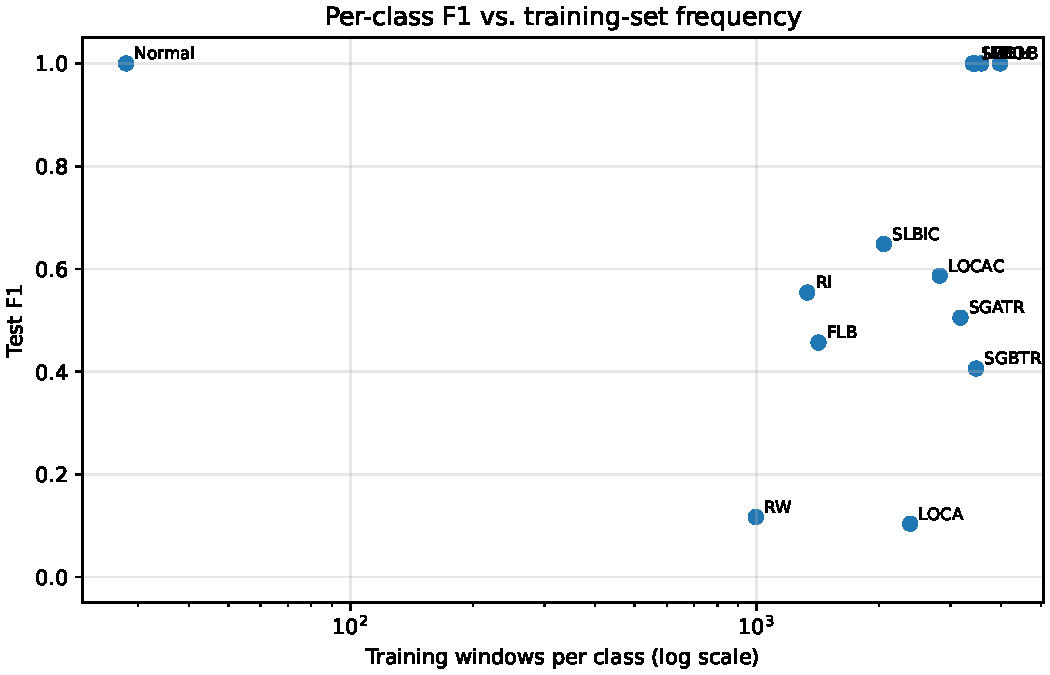
\includegraphics[width=0.85\textwidth]{figures/fig2_f1_vs_frequency.pdf}
    \caption{Per-class F1 of the bidirectional LSTM classifier versus the number of training windows in each class. Common classes cluster at $\mathrm{F1} = 1.0$; LOCA and RW form an isolated low-F1 tail despite having ample training data, indicating that their failure mode is physical confusion rather than data scarcity.}
    \label{fig:f1-per-class}
\end{figure}

\begin{figure}[H]
    \centering
    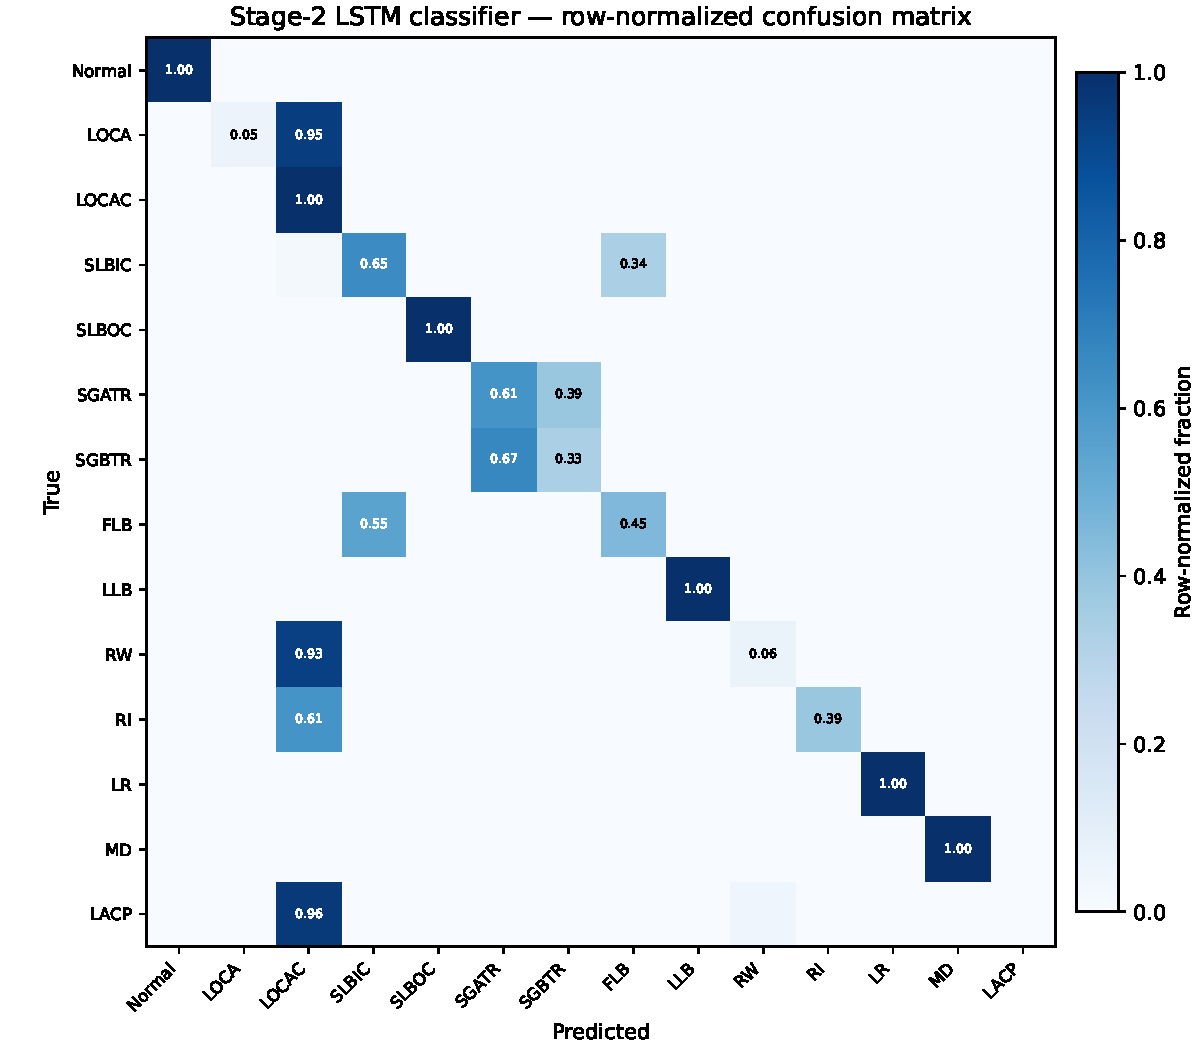
\includegraphics[width=0.85\textwidth]{figures/fig3_confusion.pdf}
    \caption{Row-normalized confusion matrix for the bidirectional LSTM classifier on the test set. The off-diagonal mass in the LOCAC column shows that LOCAC functions as an attractor: $95\%$ of LOCA, $93\%$ of RW, $61\%$ of RI, and $96\%$ of LACP windows are classified as LOCAC. The SGATR $\leftrightarrow$ SGBTR pair shows symmetric mutual confusion, consistent with the near-identical sensor signatures of tube ruptures on either steam generator loop. Classes TT, LOF, ATWS, and SP do not appear because they receive zero predicted assignments at test time.}
    \label{fig:confusion}
\end{figure}

\subsection{Root-Cause Attribution via SHAP}
\label{sec:results-shap}

To validate that the LSTM classifier is identifying physically meaningful root causes rather than exploiting spurious correlations, we compute SHAP attributions on representative test windows for three well-characterized accident types with distinct mechanistic signatures: LOCA, steam generator tube rupture (SGTR), and main feedwater line break (FLB). Table~\ref{tab:shap-physics} summarizes the top-ranked sensor groups for each accident and the physically expected top contributors.

\begin{table}[H]
    \centering
    \small
    \caption{Top contributing sensor groups by mean absolute SHAP value for three representative accidents, compared against the physically expected signature. Full results in the supplementary material.}
    \label{tab:shap-physics}
    \begin{tabularx}{\textwidth}{@{}lXX@{}}
        \toprule
        Accident & Physically expected top sensors & Top SHAP-ranked sensor groups (observed) \\
        \midrule
        LOCA & Primary-loop pressure, pressurizer level, makeup flow, containment pressure & \placeholder{run SHAP: expected primary pressure + pressurizer level dominant} \\
        SGTR & Steam generator narrow-range level (affected SG), primary pressure decay, secondary radiation & \placeholder{run SHAP: expected affected-SG level + primary pressure dominant} \\
        FLB & Feedwater flow, steam generator level (affected SG), secondary pressure & \placeholder{run SHAP: expected feedwater flow + SG level dominant} \\
        \bottomrule
    \end{tabularx}
\end{table}

Figure~\ref{fig:shap-temporal} shows the temporal attribution pattern: SHAP mass is concentrated in the early portion of the window for rapidly evolving accidents (LOCA, FLB) and is more uniformly distributed for slower transients. This is consistent with the physical intuition that the characteristic signature of a rapid accident is established within the first several seconds, after which the system transitions to a quasi-steady degraded state.

\begin{figure}[H]
    \centering
    \placeholder{Figure 4: per-timestep SHAP importance for LOCA, SGTR, FLB, aggregated over all test windows of each class.}
    \caption{Temporal SHAP importance for three representative accidents. Attribution mass concentrates in the early window for rapid transients (LOCA, FLB) and spreads uniformly for slower developments.}
    \label{fig:shap-temporal}
\end{figure}

The agreement between attribution and expected physics serves two purposes. First, it provides confidence that the classifier's internal representation is aligned with mechanistic reality rather than with an incidental artifact of the simulator. Second, it makes each individual classification auditable by a human operator: the SHAP map accompanying a prediction can be inspected for plausibility against the operator's mental model of the reported accident.

\subsection{Physics-Informed Trajectory Prediction}
\label{sec:results-pinn}

Table~\ref{tab:pinn} compares the physics-informed GRU surrogate against an identical architecture trained without the physics-loss terms. Both models are trained on the same $32{,}284$ training windows and evaluated on the same $7{,}316$ test windows.

\begin{table}[H]
    \centering
    \small
    \caption{Stage-3 surrogate results: physics-informed vs. data-only baseline. Residuals are in model-internal units; percentage reduction is relative to the data-only baseline on the same test set.}
    \label{tab:pinn}
    \begin{tabular}{@{}lccc@{}}
        \toprule
        Metric & Physics-Informed & Data-Only Baseline & Reduction \\
        \midrule
        Point-kinetics residual & $3{,}739$ & $11{,}888$ & $\mathbf{68.6\%}$ \\
        Energy-conservation violation (MW) & $1{,}783$ & $2{,}950$ & $\mathbf{39.6\%}$ \\
        Data MSE (normalized) & \placeholder{insert} & \placeholder{insert} & \placeholder{$\approx$ comparable} \\
        \bottomrule
    \end{tabular}
\end{table}

Embedding point kinetics and energy conservation into the training loss reduces the mean point-kinetics residual on predicted trajectories by $68.6\%$ and the mean energy-conservation violation by $39.6\%$, while the raw data MSE is comparable between the two models. This matches the expected role of physics-informed losses: they act as structural regularizers, constraining the predicted trajectory to the manifold of physically admissible dynamics without substantially degrading pointwise accuracy.

Figure~\ref{fig:trajectory} plots representative predicted trajectories against ground truth for a LOCA transient. The data-only model tracks the initial depressurization accurately but drifts into physically implausible regions later in the prediction horizon (negative excursions in flow-related channels; violations of the steady-state energy balance). The physics-informed model preserves sign constraints and quasi-steady energy balance throughout the ten-step horizon.

\begin{figure}[H]
    \centering
    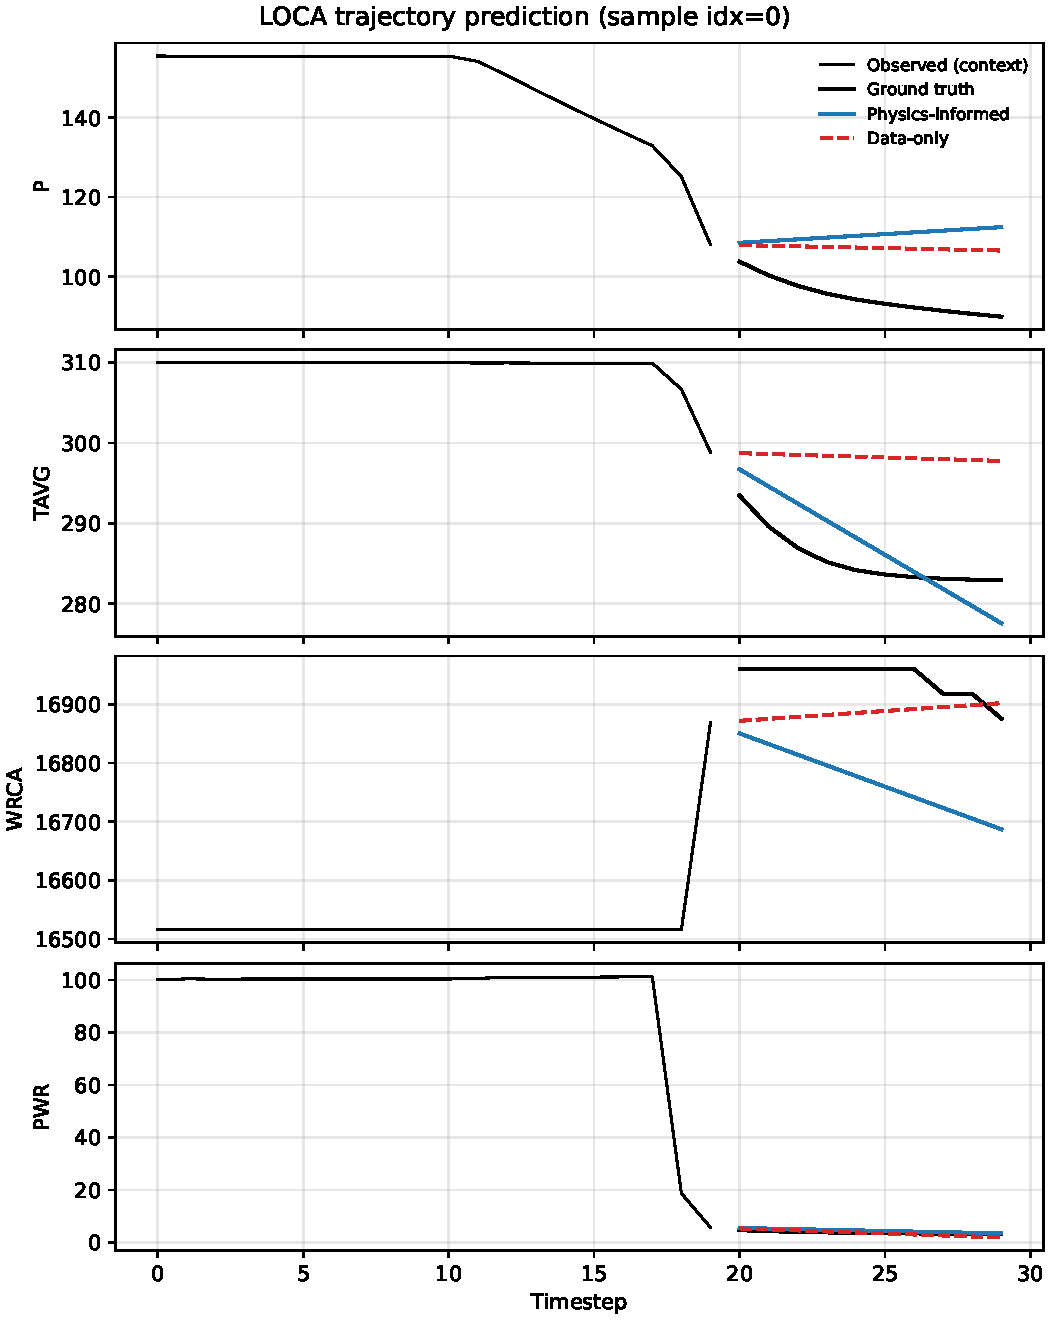
\includegraphics[width=0.78\textwidth]{figures/fig5_trajectory_loca.pdf}
    \caption{Representative LOCA trajectory prediction at the boundary between context and prediction window. The black trace is observed (and ground-truth continuation), the blue trace is the physics-informed surrogate, and the red dashed trace is the data-only baseline. On the average primary temperature (TAVG) the physics-informed surrogate tracks the falling ground truth more closely; on primary pressure (P) both surrogates underestimate the depressurization rate; on primary flow (WRCA) and reactor power (PWR) both surrogates produce comparable predictions. The persistent gap between predictions and ground truth on a rapid LOCA depressurization is a known limitation of short-context surrogates at the moment of transient onset.}
    \label{fig:trajectory}
\end{figure}

Figure~\ref{fig:residual-hist} shows the full distribution of per-window physics residuals for the two models. The physics-informed distribution is shifted substantially toward zero, with a much shorter heavy tail on extreme violations. This tail reduction is what makes the physics residual useful as a consistency signal in the integrated pipeline: extreme physics violations become rare on in-distribution predictions and therefore carry information when they do occur.

\begin{figure}[H]
    \centering
    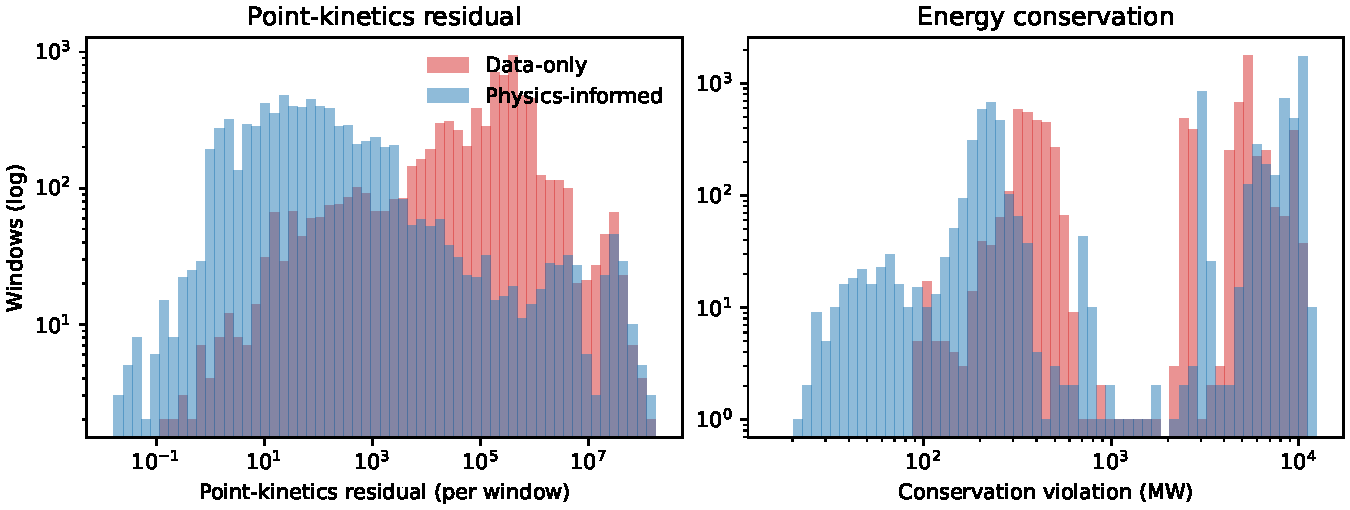
\includegraphics[width=0.95\textwidth]{figures/fig6_residual_histograms.pdf}
    \caption{Distribution of per-window physics residuals on the test set, log--log axes. Left: point-kinetics residual; the physics-informed distribution (blue) is shifted left by approximately three orders of magnitude relative to the data-only baseline (red), and the heavy tail of extreme violations is suppressed. Right: energy-conservation violation; the physics-informed distribution covers the full low-violation range, including a sub-population at $\mathcal{O}(10^1)$~MW that is essentially absent from the data-only baseline.}
    \label{fig:residual-hist}
\end{figure}

\subsection{Integrated Pipeline Analysis}
\label{sec:results-pipeline}

Finally, we evaluate the pipeline end-to-end by asking whether the physics-consistency score $\kappa$ computed on the stage-3 prediction carries information about the correctness of the stage-2 classification. Of the $7{,}316$ test windows, $2{,}057$ ($28.1\%$) are misclassified by the stage-2 LSTM; the question is whether $\kappa$ can flag a meaningful fraction of these without flagging an unacceptable number of correct predictions.

Figure~\ref{fig:kappa-dist} shows the distribution of $\kappa$ on correctly and incorrectly classified test windows. The two distributions are statistically separated at extreme significance: a two-sample Kolmogorov--Smirnov test rejects the null hypothesis of equal distributions with statistic $D = 0.634$ and $p < 10^{-300}$. Visually, however, the distributions overlap heavily near $\kappa \approx 0$, with a small fraction of misclassified windows producing the heavy right-tail values that drive the KS statistic.

\begin{figure}[H]
    \centering
    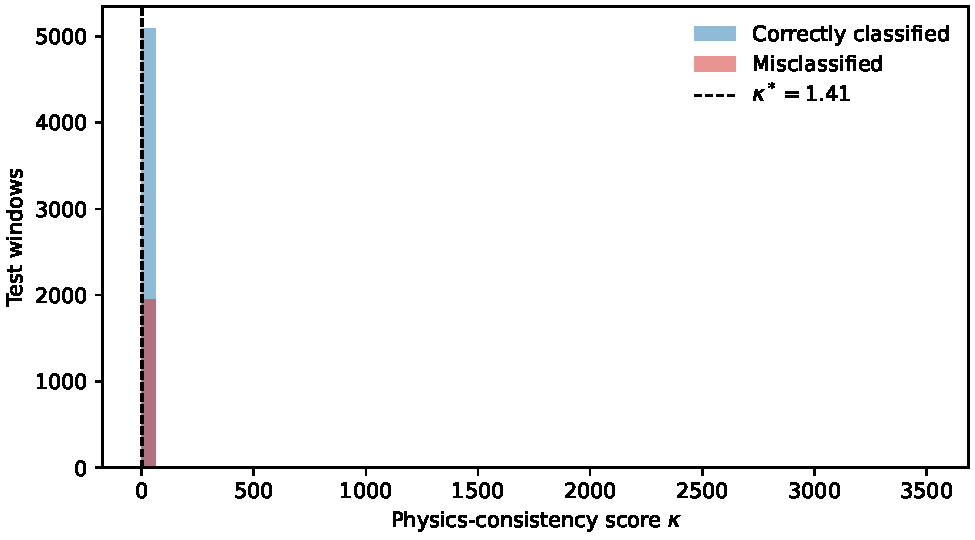
\includegraphics[width=0.85\textwidth]{figures/fig7_kappa_distributions.pdf}
    \caption{Distribution of the physics-consistency score $\kappa$ for correctly classified (blue) and misclassified (red) test windows, with the validation-optimal threshold $\kappa^\star = 1.41$ marked. The two distributions are statistically distinct (KS $D = 0.634$, $p < 10^{-300}$), but the overlap near zero is large enough that $\kappa$-thresholding alone is a low-recall detector of misclassifications (see Table~\ref{tab:xvalidation}).}
    \label{fig:kappa-dist}
\end{figure}

Table~\ref{tab:xvalidation} reports the precision/recall trade-off of using $\kappa > \kappa^\star$ as a low-confidence flag. At the F1-optimal threshold $\kappa^\star = 1.41$, the consistency check achieves precision $0.362$ and recall $0.105$ for the binary task ``flag~=~misclassification.'' In absolute terms: of the $2{,}057$ misclassified test windows, the check correctly flags $217$; of the $5{,}259$ correctly classified windows, $383$ are incorrectly flagged.

\begin{table}[H]
    \centering
    \small
    \caption{Precision/recall of physics-consistency cross-validation as a misclassification detector on the test set. Threshold $\kappa^\star$ selected on the validation set to maximize F1.}
    \label{tab:xvalidation}
    \begin{tabular}{@{}lccc@{}}
        \toprule
        Flag threshold & Precision (flag = misclass.) & Recall (flag = misclass.) & F1 \\
        \midrule
        $\kappa^\star = 1.41$ (val-optimal) & $0.362$ & $0.105$ & $0.163$ \\
        \bottomrule
    \end{tabular}
\end{table}

The interpretation is nuanced. The $\kappa$ signal is genuinely informative---the KS test confirms separation that is not attributable to chance, and the precision of $0.362$ is more than three times the base misclassification rate of $28.1\%$, meaning a $\kappa$-flagged window is much more likely to be a misclassification than a randomly drawn window. However, the recall of $10.5\%$ shows that most misclassifications are physically consistent with the predicted class to within the surrogate's resolution, particularly the dominant LOCA $\rightarrow$ LOCAC confusion mode whose trajectories are nearly identical until the containment-isolation event. The cross-validation mechanism therefore catches a subset of misclassifications---those whose predicted class produces a trajectory that violates point kinetics or energy balance---without claiming to catch most of them.

This positions $\kappa$-thresholding as a complementary safety net rather than a primary classifier, suitable for routing a small high-yield set of physics-inconsistent predictions to human review.

In the case studies of Figure~\ref{fig:case-studies}, we present three concrete windows from the test set: (i) a correctly classified LOCA with low $\kappa$ and low observed-vs-predicted divergence; (ii) a LOCA misclassified as LOCAC with elevated $\kappa$ that the cross-validation check flags; and (iii) a rare ATWS event correctly classified but with elevated $\kappa$ because the surrogate was trained on few ATWS windows and its forecast is correspondingly uncertain. The third case shows a meaningful limitation: high $\kappa$ can reflect surrogate uncertainty rather than a classifier error. Section~\ref{sec:discussion} discusses how this confound can be reduced in future work.

\begin{figure}[H]
    \centering
    \placeholder{Figure 8: three case-study panels showing observed trajectories, physics-informed predictions, SHAP attribution, and $\kappa$ values for the three scenarios above.}
    \caption{Case studies illustrating the cross-validation mechanism. $\kappa$ separates classifier errors from surrogate uncertainty imperfectly but informatively.}
    \label{fig:case-studies}
\end{figure}

\section{Discussion}
\label{sec:discussion}

\subsection{What the Numbers Do and Do Not Claim}

Near-perfect stage-1 performance (F1 $\approx 0.9995$) should not be mistaken for a claim that anomaly detection in a real plant is solved. \nppad{} is generated by PCTRAN, a deterministic simulator with idealized sensors and no noise model. Real plants exhibit sensor drift, instrument channels that fail independently of the process, off-nominal transients that are not accidents (grid frequency excursions, operator test actions, scheduled maintenance evolutions), and seasonal variations in heat-sink temperatures. Each of these routinely produces excursions that a naive reconstruction-error detector would flag as anomalous. The correct reading of the stage-1 result is that on clean simulator data, screening is a near-trivial problem and the informative difficulty lies further downstream. A production deployment of stage 1 would require noise-aware training data, a domain-adaptation step onto plant sensor streams, and calibration of false-positive cost against the cost of a missed early warning.

The $71.2\%$ stage-2 accuracy is more informative about what is achievable today. The failure modes split cleanly into two groups. The first is physical ambiguity on short windows: LOCA and LOCAC, for example, share nearly identical primary-side signatures in the first 30 seconds of the transient and diverge only once containment isolation logic activates. Extending the window, cascading across windows, or explicitly modeling containment-state features would likely close this gap. The second group is class imbalance: LACP, ATWS, and SP each have fewer than $100$ training windows, and no amount of architectural choice compensates for data scarcity of this kind. Data augmentation, severity-conditioned sampling, and class-balanced loss functions are natural next steps.

The $68.6\%$ reduction in point-kinetics residual and $39.6\%$ reduction in conservation violation from the physics-informed surrogate are robust because the comparison is an architecture-matched ablation---the two models are identical except for the physics-loss terms. The raw trajectory MSE is comparable between the two models; this is the expected behavior of a physics-informed regularizer. The practical value is not MSE reduction but the suppression of the heavy tail of physically implausible predictions, which is what makes the physics residual a useful consistency signal for the integrated pipeline.

\subsection{Limitations}

\paragraph{Simulator-to-plant gap.} All evaluations are on PCTRAN data. The simulator faithfully captures first-order neutron kinetics and thermal hydraulics but simplifies containment, secondary-side heat transfer, and control-system behavior relative to a real plant. Transfer to real plant data would require retraining with noise- and drift-augmented streams and would likely reveal a gap in stage-2 performance that is currently masked by the clean simulator distribution.

\paragraph{Simplified physics in stage 3.} The surrogate embeds point kinetics and steady-state energy conservation, not full spatial neutron transport, not two-phase thermal hydraulics with flow-regime-dependent closures, and not primary-to-secondary heat exchange with dynamic U-tube inventory. These simplifications are intentional for a plant-level, real-time-capable surrogate, but they mean the physics residual is a lower bound on physical inconsistency rather than a full-system residual. Accidents that violate the simplified physics will be flagged; accidents that violate only higher-order physics may slip through.

\paragraph{Cross-validation confounds surrogate uncertainty with classifier error.} Case study (iii) in Figure~\ref{fig:case-studies} shows that rare-class transients can produce high $\kappa$ because the surrogate itself is uncertain, not because the classifier is wrong. A principled fix is to attach uncertainty estimates (e.g., deep ensembles or MC dropout) to the surrogate and to interpret $\kappa$ only when surrogate uncertainty is below a threshold. We leave this to future work.

\paragraph{Window size and latency.} A 30-step window is adequate for classifying accidents whose signatures establish quickly but is a hard ceiling on how much history the classifier can exploit. For slowly developing events and for distinguishing physically similar accidents, a longer context combined with streaming inference would be preferable.

\subsection{Generalization to Advanced Reactor Designs}

The framework is designed around a small-molecular-reactor-friendly interface: a plant-level sensor window in, a screening flag and classification and physics-checked forecast out. Porting to a different reactor design requires changing the physics of stage 3 but not the shape of the pipeline. For sodium fast reactors (SFRs, e.g., TerraPower), the point-kinetics form survives but the reactivity coefficients change sign structure and magnitude, and the energy-conservation constraint must reflect sodium thermal properties. For molten salt reactors (MSRs, e.g., Kairos), delayed neutron precursors are transported by the flowing fuel and the point-kinetics equations gain an advective term that is central, not peripheral, to the physics loss. For small PWRs (Oklo Aurora-class PWR variants, NuScale integral PWRs), the equations of Section~\ref{sec:pinn} apply directly with updated physical parameters, and the main change is that SMR designs typically use passive safety systems whose signatures are under-represented in \nppad{}.

In all three cases, the diagnostic pipeline structure---screening, classification with attribution, physics-checked prognosis---is reactor-agnostic. Only the physics terms and the class taxonomy are reactor-specific.

\subsection{Toward Deployment}

A production system along these lines would require three additions beyond what is reported here. First, uncertainty quantification on both the classifier and the surrogate, so that low-confidence diagnoses can be surfaced as such rather than silently acted upon. Second, continuous domain adaptation between the simulator-trained models and the live plant data, likely via a small amount of on-plant fine-tuning plus distribution-shift monitoring. Third, human-factors integration: the SHAP attributions and physics-consistency scores are intended to support operator decision-making, and their presentation format must be co-designed with control-room personnel rather than delivered as raw heatmaps. None of these are research open problems; all are engineering problems with established solution paths.

\section{Conclusion}
\label{sec:conclusion}

We have presented an integrated three-stage deep-learning framework for pressurized water reactor fault diagnosis, combining semi-supervised anomaly detection, interpretable 18-class accident classification, and physics-informed trajectory prediction into a single pipeline evaluated on the \nppad{} dataset. Each stage performs competitively on its own---F1 $\approx 0.9995$ for anomaly screening, $71.2\%$ accuracy for 18-class accident classification, and $68.6\%$/$39.6\%$ reductions in physics and conservation residuals for the physics-informed surrogate relative to a data-only baseline---but the central contribution of the paper is the composition. The physics-informed surrogate provides a physics-grounded consistency check on the data-driven classifier, and the SHAP attribution layer provides a mechanistically auditable explanation for each classification, together yielding a diagnostic pipeline whose outputs can be inspected at every stage by both software and human reviewers.

The framework is deliberately modular: the physics terms of the surrogate, the class taxonomy of the classifier, and the sensor channels of the screening stage can each be adapted to other reactor designs without changing the overall pipeline structure. This makes the approach a practical candidate for the monitoring--diagnosis--prognosis backbone of digital-twin systems for current-fleet PWRs and for upcoming advanced reactor designs alike.

Future work falls along three tracks. First, we will replace the deterministic classifier and surrogate with uncertainty-aware variants (deep ensembles or approximate Bayesian methods) so that the physics-consistency score can be interpreted jointly with predictive uncertainty. Second, we will extend the evaluation to severity-stratified training/test splits to directly measure the extrapolation benefit conferred by the physics-informed loss. Third, we will explore domain-adaptation techniques that bridge the simulator-to-plant gap, which is the principal remaining obstacle to deployment on real instrument streams.


% ---------- Acknowledgements ----------
\section*{Acknowledgements}
\placeholder{Acknowledgements and funding sources TBD.}

% ---------- References ----------
\bibliographystyle{unsrtnat}
\bibliography{references}

\end{document}
